\section{rSLA language}

rSLA is a domain specific language for the service level management of cloud SLAs. rSLA follows standard ruby programming rules and implements simple production rules for the editing and processing of SLAs in a cloud environment. The complete specification on the rSLA language structure, production rules and implemented class functionality can be retrieved from \cite{rSLAspec}.

Currently, the language implements rSLA classes that are required for the management of cloud services that are leased by a real customer. The existing rSLA classes implement objects that refer to the service level objectives defined by the customer in the service level agreement.   

The rSLA language inherits semantic attributes of the WSLA specification \cite{wsla} and can be decomposed into a hierarchical tree that denotes relationships between rSLA programming objects. 
 The next paragraphs discuss the rSLA conceptual model and summarize production rules for the creation of rSLA objects. Last but not least, we describe how DSL users can create rSLA objects and customize their attributes using an editor of their choice. 

%alphabet, vocabulary, language structure, production rules 
%conceptual model on how we think about metrics, services, SLOs, Xlets

\subsection{Conceptual model}
%notion of service, metric in the abstract
In an rSLA runtime environment a service is described by its provisioning compliance levels, which in turn are decomposed into multifarious service level management elements. The rSLA language follows the semantic decomposition of the WSLA specification \cite{wsla}, where an SLA takes the form of a directed graph that has a single root vertex. The root node is connected to three vertices that denote primary branches of the hierarchical tree. 

In an rSLA tree, the root vertex represents a single SLA object. An SLA can be defined by sets of base, composite metrics and SLO objects. Figure \ref{rslaobject} illustrates programming objects of the rSLA language. Semantic connections between such objects compose an rSLA tree. Figure \ref{rslagraph} formalizes an rSLA tree as a directed graph and highlights immediate attributes of rSLA objects.

As illustrated in Figure \ref{rslagraph} an rSLA tree can be defined by a set of vertices $V$ and a set of edges $E$, where vertices represent rSLA tree branches and edges connections between such branches. The set of SLA vertices in an rSLA tree contains exactly one SLA object and one or more base metrics and service level objectives. The SLA object represents the root of the directed graph. 

There is no overlapping between rSLA language objects. Conceptually every object is related with other rSLA objects for the processing of SLA management operations. 

\begin{figure}
        \centering
        \begin{subfigure}[h]{0.5\textwidth}
                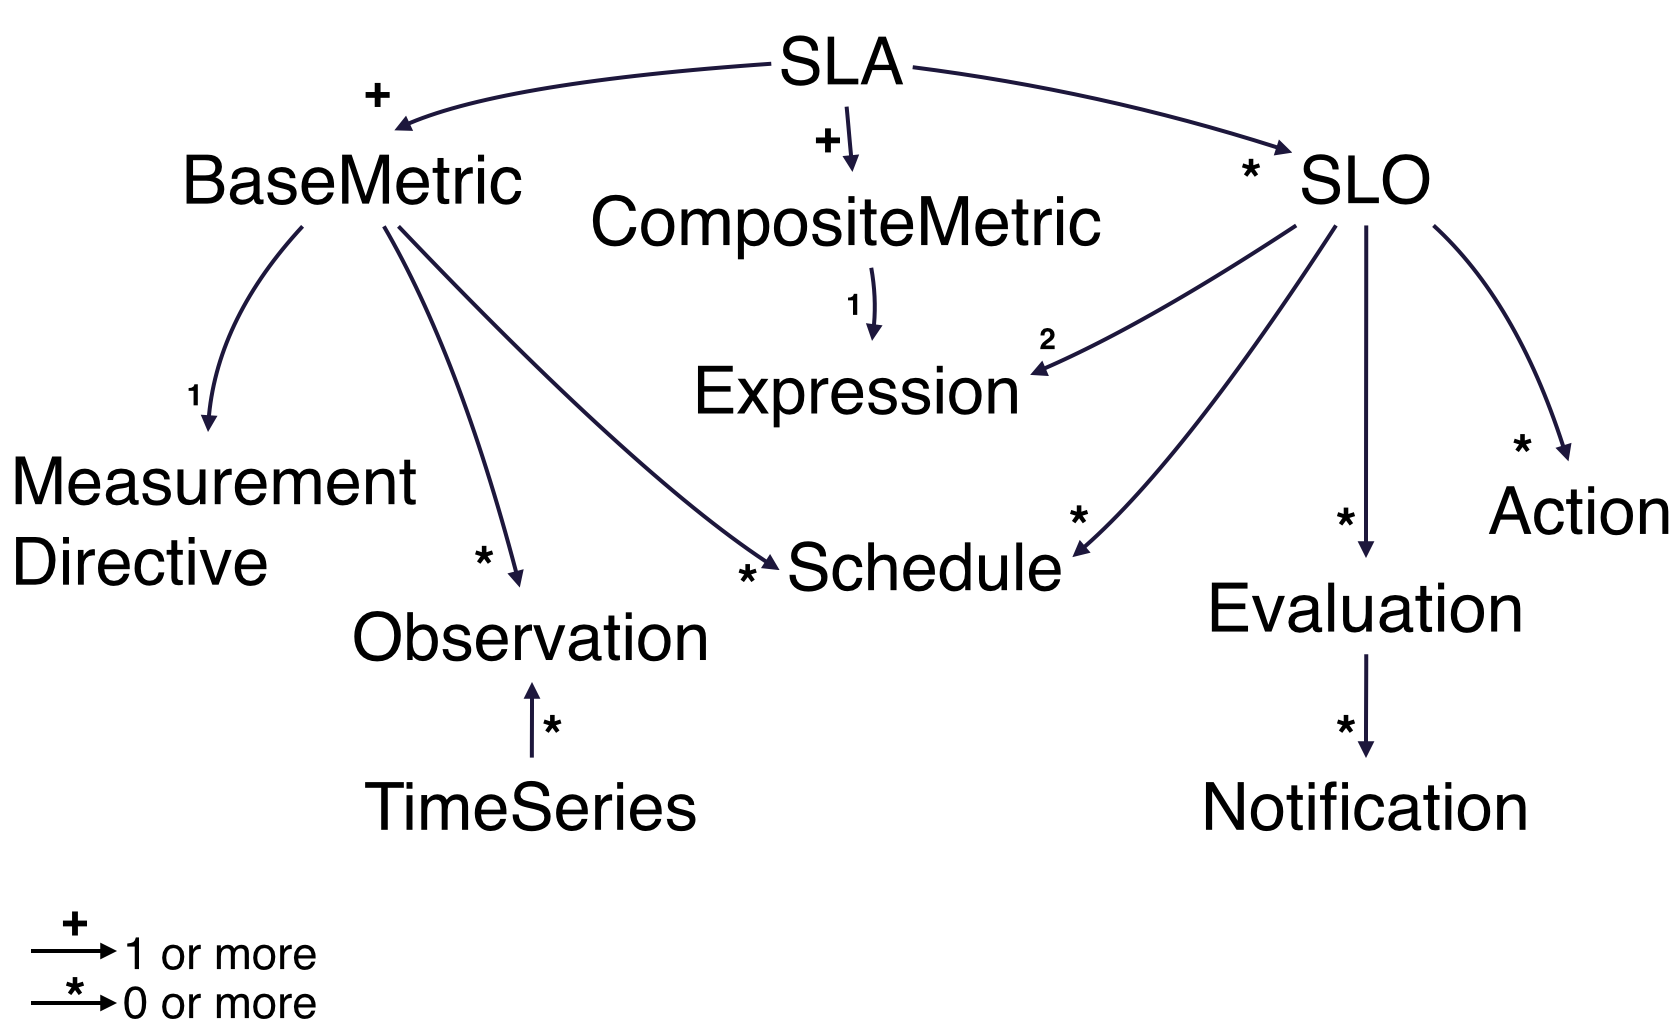
\includegraphics[height=3cm]{pics/rslaobject}
                \caption{rSLA object tree}
                \label{rslaobject}
        \end{subfigure}%
        \begin{subfigure}[h]{0.5\textwidth}
               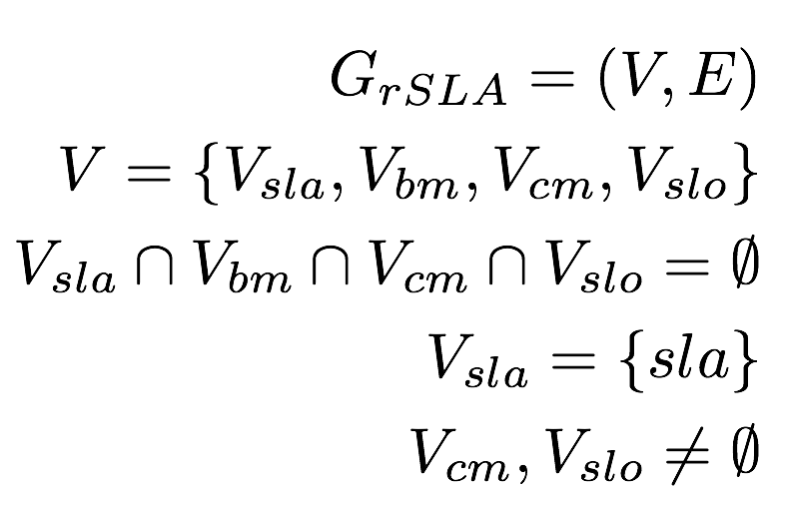
\includegraphics[height=3cm]{pics/rslagraph}
                \caption{rSLA vocabulary formalization}
                \label{rslagraph}
        \end{subfigure}
        \caption{rSLA vocabulary}\label{treegraph}
\end{figure}

Nodes that are close to the tree root in Figure \ref{rslaobject}, designate SLA branches like base, composite metrics and service level objectives. Edges between nodes are uni-directed to illustrate the rSLA tree hierarchy. The edge direction points to the nested element in the hierarchical relationship. 
Edges in Figure \ref{rslaobject} are labeled with +, * or number symbols to indicate that the multiplicity of nested objects. 

In an rSLA runtime environment, a base metric is represented by a restful endpoint that designates a URI source for reading metric data values. A base metric is also described by sets of time-series data values that are derived by the metric measurement. On the other hand, a composite metric represents the computation result from combining either a single pair of data values or multiple data value sets. 

In the rSLA alphabet nested relationships denote inclusive associations between objects. For example, an SLA includes base, composite metrics as well as SLOs. As shown in Figure \ref{rslaobject}, edges between  rSLA objects do not share same multiplicity rules. 

rSLA notification and timeSeries objects are not initially required to build and run SLA instances in a cloud environment, but they may be required while one or more SLA management tasks are processed. Such objects are created by service level management operations like statistical analysis of data coming from monitoring or automated notification reports on scheduled events of service level evaluation. 

The rSLA DSL exposes such objects as structured programming blocks that a user can edit and modify according to specific needs. The use and characteristics of rSLA programming blocks are analyzed in Section \ref{editing}. Moreover, a user can introduce new elements in the rSLA vocabulary by integrating their definition in the rSLA programming library. 

\subsection{rSLA language production rules}

The rSLA DSL uses production rules in Backus-Naur form (BNF) notation to describe the syntax of rSLA programming blocks. As we discuss in the next section, ruby programming blocks represent the editing rules of the rSLA language. The description of rSLA blocks in BNF notation exemplifies how to use and extend such structures with the rSLA programming library.

In the BNF grammar, every rule is decomposed into another set of rules and literals. The symbol "::=" refers to \textit{is defined} or \textit{is produced by}. Literal or terminal symbols are denoted as "literal" and non-literal symbols are enclosed in brackets $<>$.

Grammar \ref{slobnf} illustrates an excerpt of the rSLA BNF production rules for the generation of an SLO object. Service level objectives (SLOs) describe promises from a provider to a customer with respect to service provisioning levels\cite{wsla}. An SLA is defined by one or more SLOs. The right side of Line 1 in Grammar \ref{slobnf} summarizes the block of statements that the rSLA DSL requires as input for the creation of a new SLO object.
\begin{lstlisting}[caption= Service level objective (SLO) production rules, label=slobnf]
<SLO> ::= "slo" "do" <name> <precondition> <objective> <schedule> "end" ;
<name>::= "name" <string> ;
<precondition>::= <expression> ;
<objective> ::= <expression> ;
<schedule> ::= "schedule" "do" <frequency> <unit> <method> "end";
\end{lstlisting} 
An SLO object has a name that is represented by a string. An SLO is also specified by a precondition and by an objective that in the rSLA grammar are denoted with the symbol $<$expression$>$. 
The rSLA language supports the free formation of valid ruby statements. Free-formatted statements define expression objects. In the rSLA grammar an expression object is represented as a non-literal symbol that is further refined into statement combinations. The decomposition of a non-literal expression may produce various statements that associate both literal and non-literal symbols . 

An rSLA expression may refer to other rSLA objects and may define numerical and logical expressions for their description. Section \ref{editing} provides an $<$expression$>$ example for the creation of a new SLO object using an rSLA programming block.

An SLO object also embeds in its definition one or more schedules for its evaluation. In the rSLA grammar, a schedule represents a non-literal symbol that is syntactically and contextually decomposed into the non-literal symbols of frequency, unit and method. Frequency determines the schedule periodicity, thus how often a scheduler triggers execution tasks with respect to a schedule. The schedule unit determines in time units the intervals to fire schedule events. The non-literal method describes how to run tasks of the defined schedule. A method may consist of either literal or non-literal statements.

\subsection{rSLA editing}\label{editing}

The rSLA DSL exposes ruby programming blocks for the production of SLO objects. A DSL user can edit and extend such programming blocks according to domain specific needs. An example of such a ruby programming block for the creation of an SLO object is illustrated by rSLA coding block \ref{slob}.
\begin{lstlisting}[caption=SLO definition, label=slob]
slo do
     name "CpuUtil"
     precondition do CPUutilization.value<15 end
     objective do CPUmetric1.value<10 end
     schedule do
      	frequency "30"
    	unit "m"
    	method "every"
    end
end	
\end{lstlisting}

The SLO definition of \ref{slob} provides a configuration sample for the generation of SLO objects with the rSLA language. In the ruby block, precondition and objective expressions are defined using both non-literal and literal symbols. In this case, non-literal terms refer to other rSLA objects. For example in the precondition statement, an expression is defined by stating a condition for the numeric value of a CPUutilization rSLA object. Similarly, the objective sets a condition for the numeric value of a CPUmetric object.

The programming logic between a precondition and an objective expression is sequential and can be summarized by the following steps:

\begin{lstlisting}[language=Ruby, basicstyle=\small\normalfont\sffamily, breaklines=true,  captionpos=b, mathescape=true, caption=rSLA SLO precondition-objective logic, label=ifelse, numbers=left, numbersep=5pt, numberstyle=\tiny]
if $eval(Precondition)\rightarrow \neg Precondition$ then $SLO_{healthy}$ = true
 elsif $((\neg \exists Precondition)\lor(Precondition=true)) \wedge eval(Objective) \rightarrow$ true
 then $SLO_{healthy}$=true 
 end
else $SLO_{healthy}$=false
  end
\end{lstlisting}

On SLO evaluation, the rSLA engine will evaluate first the precondition statement block. If the logical outcome from the execution of the precondition block is false, the SLO is healthy. In case the precondition is true or if there is no precondition block, the rSLA runtime will proceed with the evaluation of the objective block. If the logical outcome from processing statements of the objective block is true, then the SLO is healthy. Otherwise the SLO evaluation indicates not-healthy. A non-healthy SLO may result into a violation.